% ==============================================================================
% Relatório AutoML v3.0 - Equipe 9
% Universidade do Estado do Amazonas (UEA)
% Disciplina: Ciência de Dados
% Equipe 9: FLAML e LightAutoML
% ==============================================================================

\documentclass[11pt, a4paper, oneside]{article}

% ==============================================================================
% Encoding e idioma
% ==============================================================================
\usepackage[T1]{fontenc}
\usepackage[utf8]{inputenc}
\usepackage[brazil]{babel}

% ==============================================================================
% Layout
% ==============================================================================
\usepackage{geometry}
\usepackage{lmodern}
\usepackage{microtype}
\usepackage{setspace}
\usepackage{parskip}
\usepackage{fancyhdr}
\usepackage{lastpage}
\usepackage{titlesec}
\usepackage{tocloft}
\usepackage{float}
\usepackage{xurl}
\usepackage{amsmath}

% ==============================================================================
% Gráficos, cores e diagramas
% ==============================================================================
\usepackage{graphicx}
\usepackage{xcolor}
\usepackage{tikz}

% ==============================================================================
% Tabelas e listas
% ==============================================================================
\usepackage{booktabs}
\usepackage{longtable}
\usepackage{tabularx}
\usepackage{array}
\usepackage{multirow}
\usepackage{colortbl}
\usepackage{ragged2e}
\usepackage{enumitem}

% ==============================================================================
% Caixas e código
% ==============================================================================
\usepackage{tcolorbox}
\tcbuselibrary{skins,breakable}
\usepackage{hyperref}

% ==============================================================================
% Geometria da página
% ==============================================================================
\geometry{
  a4paper,
  top=25mm, bottom=25mm,
  left=25mm, right=20mm,
  headheight=50mm, headsep=6mm,
  footskip=12mm
}

\graphicspath{{./}{../../diagrams/}}
\setlength{\emergencystretch}{3em}
\setlength{\hfuzz}{2pt}
\setlength{\LTleft}{0pt}
\setlength{\LTright}{0pt}
\setlength{\tabcolsep}{4pt}
\Urlmuskip=0mu plus 2mu\relax

% ==============================================================================
% Cores (identidade UEA)
% ==============================================================================
\definecolor{ueagreen}{RGB}{26, 92, 42}
\definecolor{ueamint}{RGB}{74, 158, 107}
\definecolor{ueagray}{RGB}{88, 88, 90}
\definecolor{ueadark}{RGB}{30, 30, 30}
\definecolor{uealight}{RGB}{240, 248, 243}
\definecolor{tablehead}{RGB}{26, 92, 42}
\definecolor{tableheadlight}{RGB}{220, 240, 228}
\definecolor{tablealt}{RGB}{242, 250, 245}
\definecolor{alertcolor}{RGB}{180, 100, 0}
\definecolor{alertlight}{RGB}{255, 235, 210}
\definecolor{infolight}{RGB}{235, 248, 242}

% ==============================================================================
% Hyperref
% ==============================================================================
\hypersetup{
  colorlinks  = true,
  linkcolor   = ueagreen,
  urlcolor    = ueamint,
  citecolor   = ueagray,
  pdftitle    = {Relatório AutoML v3.0 - Equipe 9 - UEA Ciência de Dados},
  pdfauthor   = {Ana Beatriz Maciel Nunes, Fernando Luiz Da Silva Freire, Juliana Ballin Lima},
  pdfsubject  = {AutoML: FLAML e LightAutoML aplicados ao dataset ANP},
  pdfkeywords = {AutoML, FLAML, LightAutoML, ANP, Combustíveis, Ciência de Dados, UEA}
}

% ==============================================================================
% Tipos de coluna
% ==============================================================================
\newcolumntype{J}[1]{>{\justifying\arraybackslash\small}p{#1}}
\newcolumntype{L}[1]{>{\raggedright\arraybackslash\small}p{#1}}
\newcolumntype{C}[1]{>{\centering\arraybackslash\small}p{#1}}
\newcolumntype{Y}{>{\justifying\arraybackslash\small}X}
\renewcommand{\arraystretch}{1.25}

% ==============================================================================
% Formatação de seções
% ==============================================================================
\titleformat{\section}[block]
  {\Large\bfseries\color{ueagreen}}
  {\thesection}{1em}{}
  [\vspace{1pt}{\color{ueamint}\hrule height 1.5pt}\vspace{4pt}]

\titleformat{\subsection}[block]
  {\large\bfseries\color{ueagreen}}
  {\thesubsection}{1em}{}

\titleformat{\subsubsection}[block]
  {\normalsize\bfseries\color{ueagray}}
  {\thesubsubsection}{1em}{}

\titlespacing{\section}{0pt}{18pt}{6pt}
\titlespacing{\subsection}{0pt}{12pt}{4pt}
\titlespacing{\subsubsection}{0pt}{8pt}{2pt}

% ==============================================================================
% Helpers de logo
% ==============================================================================
\newcommand{\uealogo}{%
  \IfFileExists{uea-logo.png}{%
    \raisebox{-3mm}{%
      \begin{tikzpicture}
        \clip[rounded corners=1.4mm] (0,0) rectangle (27.65mm,14mm);
        \node[inner sep=0pt, anchor=south west] at (0,0)
          {
\includegraphics[height=14mm]{uea-logo.png}};
      \end{tikzpicture}%
    }%
  }{\textbf{\color{ueagreen}UEA}}%
}

\newcommand{\projlogo}{%
  \IfFileExists{../../diagrams/logo.png}{%
    
\includegraphics[height=12mm]{../../diagrams/logo.png}%
  }{\textcolor{ueagreen}{\small\textbf{ANP}}}%
}

% ==============================================================================
% Cabeçalho e rodapé
% ==============================================================================
\pagestyle{fancy}
\fancyhf{}
\fancyhead[L]{\uealogo}
\fancyhead[C]{\textcolor{ueagray}{\small Ciência de Dados $\cdot$ AutoML}}
\fancyhead[R]{\vspace{-2mm}\projlogo}
\fancyfoot[L]{\textcolor{ueagray}{\small UEA $\cdot$ Equipe 9}}
\fancyfoot[C]{\textcolor{ueagray}{\small\textbullet\quad\thepage\quad\textbullet}}
\fancyfoot[R]{\textcolor{ueagray}{\small v3.0}}
\renewcommand{\headrulewidth}{0.6pt}
\renewcommand{\headrule}{%
  \hbox to\headwidth{\color{ueagreen}\leaders\hrule height \headrulewidth\hfill}}
\renewcommand{\footrulewidth}{0.3pt}
\renewcommand{\footrule}{%
  \hbox to\headwidth{\color{ueagray}\leaders\hrule height \footrulewidth\hfill}}

% ==============================================================================
% Caixas utilitárias
% ==============================================================================
\newtcolorbox{notebox}{
  colback=alertlight,
  colframe=alertcolor,
  arc=2mm,
  boxrule=1.5pt,
  leftrule=4pt,
  sharp corners,
  breakable,
  enhanced
}

\newtcolorbox{infobox}{
  colback=infolight,
  colframe=ueamint,
  arc=2mm,
  boxrule=1.5pt,
  leftrule=4pt,
  sharp corners,
  breakable,
  enhanced
}

\newcommand{\thead}[1]{\cellcolor{tablehead}\color{white}\small\bfseries\shortstack[c]{#1}}
\newcommand{\taltrow}{\rowcolor{tablealt}}

% ==============================================================================
\begin{document}
% ==============================================================================

% ==============================================================================
% Capa
% ==============================================================================
\hypersetup{pageanchor=false}
\newgeometry{
  top=10mm, bottom=10mm,
  left=25mm, right=20mm,
  noheadfoot
}
\begin{titlepage}
  \thispagestyle{empty}
  \pagecolor{ueagreen}
  \color{white}
  \vspace*{\fill}

  \begin{center}
    \IfFileExists{uea-logo.png}{%
      \begin{tikzpicture}
        \clip[rounded corners=2.4mm] (0,0) rectangle (47.4mm,24mm);
        \node[inner sep=0pt, anchor=south west] at (0,0)
          {
\includegraphics[height=24mm]{uea-logo.png}};
      \end{tikzpicture}
    }{%
      {\fontsize{28}{34}\selectfont\textbf{UEA}}
    }\\[3mm]
    {\fontsize{15}{19}\selectfont Universidade do Estado do Amazonas}\\[1mm]
    {\fontsize{14}{18}\selectfont Escola Superior de Tecnologia}
  \end{center}

  \vspace{7mm}
  \noindent\textcolor{ueamint}{\rule{\textwidth}{1.5pt}}\\[4mm]
  {\fontsize{21}{26}\selectfont\textbf{Comparação de Ferramentas AutoML}}\\[3mm]
  {\fontsize{16}{21}\selectfont\textbf{FLAML e LightAutoML}}\\[3mm]
  {\fontsize{13}{17}\selectfont Aplicadas ao Dataset de Combustíveis ANP}\\[2mm]
  \noindent\textcolor{white}{\rule{\textwidth}{0.5pt}}

  \vspace{7mm}

  \begin{tabularx}{\textwidth}{@{}L{4cm} Y@{}}
    \textbf{Disciplina:}  & Ciência de Dados \\[2mm]
    \textbf{Equipe:}      & 9 \\[2mm]
    \textbf{Ferramentas:} & FLAML e LightAutoML \\[2mm]
    \textbf{Versão:}      & 3.0 \\[2mm]
    \textbf{Data:}        & 31 de maio de 2026 \\[2mm]
    \textbf{Integrantes:} & Ana Beatriz Maciel Nunes \\
                          & Fernando Luiz Da Silva Freire \\
                          & Juliana Ballin Lima \\
  \end{tabularx}

  \vspace{8mm}

  \begin{center}
    \IfFileExists{../../diagrams/logo.png}{%
      
\includegraphics[height=20mm]{../../diagrams/logo.png}
    }{}
  \end{center}

  \vspace{3mm}
  \noindent\textcolor{ueamint}{\rule{\textwidth}{0.5pt}}\\[2mm]
  \begin{center}
  \begin{minipage}{0.92\textwidth}
  \centering
  {\small Este relatório apresenta o conjunto completo da atividade de comparação de
  ferramentas AutoML: Parte 1 (teoria), Parte 2 (dataset), Parte 3 (FLAML),
  Parte 4 (LightAutoML) e Parte 5 (reflexão e comparação), como entrega final
  da atividade da disciplina de Ciência de Dados na UEA.}
  \end{minipage}

  \vspace{3mm}
  {\small \textcopyright{} 2026 Equipe 9, Ciência de Dados, UEA. Uso acadêmico.}

  \vspace{2mm}
  {\small UEA $\cdot$ Equipe 9 $\bullet$ v3.0}
  \end{center}
  \vspace*{\fill}
\end{titlepage}
\restoregeometry
\hypersetup{pageanchor=true}
\setcounter{page}{1}

\pagecolor{white}
\color{ueadark}

% ==============================================================================
% Histórico de versões
% ==============================================================================
\thispagestyle{fancy}
\section*{Histórico de Versões}
\addcontentsline{toc}{section}{Histórico de Versões}

\begin{tabularx}{\textwidth}{@{}L{1.8cm} L{2.8cm} L{4cm} Y@{}}
  \toprule
  \thead{Versão} & \thead{Data} & \thead{Autores} & \thead{Descrição} \\
  \midrule
  1.0 & 26/05/2026 & Equipe 9 & Criação inicial do relatório. Parte 1: explicação teórica sobre AutoML. Parte 2: descrição do dataset ANP. \\
  \taltrow 2.0 & 30/05/2026 & Equipe 9 & Segunda entrega. Parte 3: aplicação da primeira ferramenta AutoML, FLAML, ao problema de regressão do preço médio da gasolina C. \\
  3.0 & 31/05/2026 & Equipe 9 & Entrega final. Parte 4: aplicação da segunda ferramenta AutoML, LightAutoML. Parte 5: reflexão crítica e comparação entre as duas ferramentas. \\
  \bottomrule
\end{tabularx}

\vspace{6mm}

\begin{infobox}
\textbf{Organização dos relatórios da atividade:}
\begin{itemize}[leftmargin=1.2cm, topsep=2pt, itemsep=2pt]
  \item \textbf{v1.0}: Parte 1 - Explicação teórica sobre AutoML; Parte 2 - Descrição do dataset.
  \item \textbf{v2.0}: Parte 3 - Aplicação da primeira ferramenta AutoML (FLAML).
  \item \textbf{v3.0} (este documento): Parte 4 - Aplicação da segunda ferramenta (LightAutoML); Parte 5 - Reflexão e comparação das ferramentas. Inclui também as partes anteriores para completude.
\end{itemize}
\end{infobox}

\newpage

% ==============================================================================
% Sumário
% ==============================================================================
\tableofcontents
\newpage

% ==============================================================================
% Resumo executivo
% ==============================================================================
\section*{Resumo Executivo}
\addcontentsline{toc}{section}{Resumo Executivo}

Este relatório consolida a comparação entre \textbf{FLAML} e \textbf{LightAutoML}
na previsão do preço médio mensal da gasolina C por UF, usando o dataset tratado da
ANP entre janeiro de 2021 e dezembro de 2025. As duas ferramentas foram avaliadas
com a mesma variável-alvo, a mesma divisão treino e teste, a mesma semente aleatória
e a mesma métrica principal, RMSE.

\begin{table}[H]
\centering
\small
\setlength{\tabcolsep}{4.5pt}
\begin{tabularx}{\textwidth}{@{}Y C{2cm} C{2cm} C{2cm} C{2.4cm}@{}}
  \toprule
  \thead{Ferramenta} & \thead{RMSE} & \thead{MAE} & \thead{R²} & \thead{Tempo} \\
  \midrule
  \taltrow FLAML & 0,1148 & 0,0819 & 0,9693 & 60,78s \\
  LightAutoML & 0,1134 & 0,0888 & 0,9701 & 73,94s \\
  \bottomrule
\end{tabularx}
\caption{Resumo dos principais resultados no conjunto de teste.}
\label{tab:resumo-executivo}
\end{table}

\begin{infobox}
\textbf{Conclusão executiva:} as duas ferramentas apresentaram desempenho praticamente
equivalente. A LightAutoML teve leve vantagem em RMSE e R², enquanto a FLAML teve
melhor MAE, melhor MAPE, menor tempo de execução e maior transparência operacional.
Para iniciantes, a recomendação da equipe é a FLAML. Para cenários com necessidade
de pipelines mais automatizados e multiníveis, a LightAutoML é uma alternativa robusta.
\end{infobox}

\textbf{Principais evidências coletadas:}
\begin{itemize}[leftmargin=1.5cm, itemsep=4pt]
  \item Os experimentos foram executados por scripts reprodutíveis em \texttt{src/flaml\_analysis.py} e \texttt{src/lightautoml\_analysis.py}.
  \item As métricas e previsões da FLAML estão registradas nas tabelas de saída do experimento.
  \item As métricas e previsões da LightAutoML estão registradas nas tabelas de saída do experimento.
  \item Os gráficos de valores reais contra previstos, importância de atributos e erros regionais estão em \texttt{outputs/figures/}.
  \item As colunas com risco de vazamento de dados foram removidas antes do treinamento nas duas ferramentas.
\end{itemize}

\newpage

% ==============================================================================
% SEÇÃO 1 - Explicação Teórica sobre AutoML
% ==============================================================================
\section{Explicação Teórica sobre AutoML}
\label{sec:automl-teoria}

\begin{infobox}
Esta seção responde às questões teóricas solicitadas na atividade sobre AutoML, com
base nos slides disponibilizados na nota da disciplina
(\url{https://classroom.google.com/u/1/c/NzkzOTU2MDI1NjE4}) e com base em
pesquisa bibliográfica e compreensão conceitual da equipe.
\end{infobox}

% ------------------------------------------------------------------------------
\subsection{O que é AutoML?}
\label{sec:o-que-e-automl}
% ------------------------------------------------------------------------------

AutoML (Automated Machine Learning) é o conjunto de técnicas, ferramentas e processos
que automatizam etapas repetitivas e técnicas do ciclo de desenvolvimento de modelos
de Machine Learning. O objetivo central é reduzir o esforço manual necessário para
construir pipelines de ML de qualidade, desde a preparação dos dados até a seleção e
otimização do modelo final.

Diferentemente da abordagem tradicional, em que o cientista de dados realiza
manualmente cada escolha do pipeline, como a seleção do algoritmo, o ajuste de
hiperparâmetros e a engenharia de atributos, o AutoML executa essas etapas de forma
sistemática e automatizada. Isso é possível graças a técnicas como busca em espaço de
hiperparâmetros, otimização bayesiana, meta-aprendizado e avaliação cruzada automática.

O AutoML surgiu como resposta à crescente demanda por aplicações de ML em diferentes
domínios e à escassez de especialistas com domínio técnico profundo. Ferramentas como
FLAML, LightAutoML, AutoGluon, H2O AutoML e PyCaret representam implementações
práticas desse conceito, cada uma com diferentes abordagens e focos.

% ------------------------------------------------------------------------------
\subsection{Etapas de ML que podem ser automatizadas}
\label{sec:etapas-automatizadas}
% ------------------------------------------------------------------------------

Diversas etapas do ciclo de Machine Learning podem ser total ou parcialmente
automatizadas por ferramentas AutoML:

\begin{itemize}[leftmargin=1.5cm, itemsep=4pt]
  \item \textbf{Pré-processamento de dados:} imputação de valores ausentes, normalização e padronização de variáveis numéricas, codificação de variáveis categóricas (one-hot, label encoding) e detecção de tipos de dados.
  \item \textbf{Engenharia de atributos:} criação e transformação de features, seleção automática de atributos relevantes e redução de dimensionalidade.
  \item \textbf{Seleção de algoritmos:} comparação automática entre múltiplos algoritmos de ML (regressão linear, árvores de decisão, gradient boosting, redes neurais, entre outros).
  \item \textbf{Ajuste de hiperparâmetros:} busca automática das melhores configurações de cada modelo por meio de grid search, random search ou otimização bayesiana.
  \item \textbf{Avaliação e validação:} aplicação automática de validação cruzada (cross-validation), cálculo de métricas de desempenho e seleção do melhor modelo com base nos resultados.
  \item \textbf{Ensemble de modelos:} combinação automática de múltiplos modelos para melhorar o desempenho final (stacking, bagging, blending).
  \item \textbf{Geração de relatórios:} criação automática de resumos com métricas, importância de atributos e leaderboards comparativos.
\end{itemize}

% ------------------------------------------------------------------------------
\subsection{Etapas que ainda dependem da análise humana}
\label{sec:etapas-humanas}
% ------------------------------------------------------------------------------

Apesar do alto grau de automação, várias etapas do processo de ML ainda dependem
fundamentalmente da análise e julgamento humanos:

\begin{itemize}[leftmargin=1.5cm, itemsep=4pt]
  \item \textbf{Definição do problema:} identificar qual pergunta se quer responder, qual é a variável-alvo e que tipo de problema se trata (classificação, regressão, clustering).
  \item \textbf{Coleta e curadoria de dados:} obter, limpar e organizar os dados de forma adequada ao problema. A qualidade dos dados é responsabilidade humana.
  \item \textbf{Definição de métricas de avaliação:} escolher a métrica mais adequada ao contexto do negócio ou da pesquisa.
  \item \textbf{Interpretação dos resultados no contexto do domínio:} entender o significado prático das previsões do modelo e validar se fazem sentido no contexto real.
  \item \textbf{Avaliação ética e de vieses:} identificar e mitigar vieses presentes nos dados ou nos modelos.
  \item \textbf{Validação com especialistas do domínio:} verificar se os resultados são coerentes com o conhecimento especializado da área.
  \item \textbf{Implantação e monitoramento em produção:} decidir como integrar o modelo ao sistema real e como monitorar seu desempenho ao longo do tempo.
\end{itemize}

% ------------------------------------------------------------------------------
\subsection{Principais vantagens do AutoML}
\label{sec:vantagens}
% ------------------------------------------------------------------------------

O uso de ferramentas AutoML traz diversas vantagens práticas e estratégicas:

\begin{itemize}[leftmargin=1.5cm, itemsep=4pt]
  \item \textbf{Redução do tempo de desenvolvimento:} o processo que levaria dias ou semanas de experimentação manual pode ser realizado em horas.
  \item \textbf{Democratização do ML:} permite que analistas e pesquisadores utilizem técnicas avançadas sem dominar todos os aspectos matemáticos e computacionais.
  \item \textbf{Exploração sistemática do espaço de modelos:} o AutoML explora combinações de algoritmos e hiperparâmetros de forma mais abrangente do que um humano poderia fazer manualmente.
  \item \textbf{Reprodutibilidade:} o processo automatizado garante que os experimentos possam ser replicados com os mesmos resultados.
  \item \textbf{Redução de erros humanos:} evita descuidos comuns na configuração manual de pipelines, como vazamento de dados e comparação inadequada de modelos.
  \item \textbf{Baseline rápido:} permite obter um modelo de referência de qualidade rapidamente.
\end{itemize}

% ------------------------------------------------------------------------------
\subsection{Riscos e limitações do AutoML}
\label{sec:riscos}
% ------------------------------------------------------------------------------

O AutoML não é uma solução universal e apresenta riscos e limitações importantes:

\begin{itemize}[leftmargin=1.5cm, itemsep=4pt]
  \item \textbf{Interpretabilidade reduzida:} os modelos gerados automaticamente, especialmente ensembles complexos, podem ser difíceis de interpretar.
  \item \textbf{Alto custo computacional:} a busca automática por melhores modelos pode demandar muito tempo e recursos computacionais.
  \item \textbf{Risco de overfitting:} sem uma configuração adequada da validação, os modelos podem se ajustar excessivamente aos dados de treino.
  \item \textbf{Dependência da qualidade dos dados:} o AutoML não corrige problemas fundamentais nos dados de entrada.
  \item \textbf{Caixa-preta:} a automação pode obscurecer as escolhas feitas pelo sistema, dificultando o diagnóstico de problemas.
  \item \textbf{Limitações no domínio do problema:} nem sempre o AutoML encontra o melhor modelo para problemas muito específicos.
\end{itemize}

% ------------------------------------------------------------------------------
\subsection{AutoML substitui o cientista de dados?}
\label{sec:substitui}
% ------------------------------------------------------------------------------

\textbf{Não.} O AutoML é uma ferramenta que potencializa o trabalho do cientista de
dados, mas não o substitui. As razões são diversas:

Em primeiro lugar, o AutoML automatiza tarefas técnicas e repetitivas, mas não é
capaz de definir o problema correto, compreender o contexto do negócio, avaliar a
qualidade e relevância dos dados nem interpretar os resultados à luz do conhecimento
especializado do domínio.

Em segundo lugar, o uso irresponsável de AutoML sem compreensão do processo pode
levar a modelos tendenciosos, com vazamento de dados ou com métricas infladas que
não refletem o desempenho real.

Em terceiro lugar, a implantação de modelos em produção, o monitoramento de desvios
ao longo do tempo e as decisões éticas sobre uso de algoritmos em contextos sensíveis
exigem julgamento humano que nenhuma ferramenta automatizada possui.

\begin{infobox}
\textbf{Conclusão:} AutoML é um acelerador poderoso no toolkit do cientista de dados.
Ele elimina parte do trabalho repetitivo, permite explorar mais alternativas em menos
tempo e facilita a construção de baselines rápidos. Mas o papel do cientista de dados
permanece insubstituível nas etapas que exigem julgamento, contexto e responsabilidade.
\end{infobox}

\newpage

% ==============================================================================
% SEÇÃO 2 - Descrição do Dataset
% ==============================================================================
\section{Descrição do Dataset}
\label{sec:dataset}

% ------------------------------------------------------------------------------
\subsection{Identificação e Fonte}
\label{sec:dataset-fonte}
% ------------------------------------------------------------------------------

\begin{tabularx}{\textwidth}{@{}L{4.5cm} Y@{}}
  \toprule
  \textbf{Campo} & \textbf{Informação} \\
  \midrule
  \taltrow \textbf{Nome} & Dataset ANP - Análise de Preços e Volumes de Combustíveis (2021-2025) \\
  \textbf{Fonte} & Agência Nacional do Petróleo, Gás Natural e Biocombustíveis (ANP), bases públicas: Série Histórica do Levantamento de Preços e Vendas de Derivados de Petróleo e Biocombustíveis \\
  \taltrow \textbf{Disponibilidade} & Público, disponibilizado pela ANP no portal de dados abertos \\
  \textbf{Período} & Janeiro de 2021 a dezembro de 2025 \\
  \taltrow \textbf{Granularidade} & Mensal por Unidade Federativa (UF) \\
  \textbf{Arquivo processado} & \texttt{data/processed/dataset\_anp\_pca\_mds\_2021\_2025.csv} \\
  \bottomrule
\end{tabularx}

\vspace{6mm}

O dataset foi construído a partir do cruzamento entre duas bases públicas da ANP: a
série histórica de preços médios de revenda de combustíveis e os registros de volume
vendido (em m³) de derivados de petróleo e biocombustíveis. O merge foi realizado por
mês e sigla de UF, garantindo a inclusão de todas as 27 unidades federativas.

% ------------------------------------------------------------------------------
\subsection{Estrutura dos Dados}
\label{sec:dataset-estrutura}
% ------------------------------------------------------------------------------

\begin{tabularx}{\textwidth}{@{}L{5.5cm} L{2.5cm} Y@{}}
  \toprule
  \thead{Atributo} & \thead{Tipo} & \thead{Descrição} \\
  \midrule
  \taltrow \texttt{mes\_ano} & Data & Mês e ano de referência da observação (formato YYYY-MM-01) \\
  \texttt{uf} & Categórico & Sigla da Unidade Federativa (ex.: AM, SP, RJ) \\
  \taltrow \texttt{uf\_nome} & Categórico & Nome completo da UF (ex.: AMAZONAS) \\
  \texttt{regiao} & Categórico & Região geográfica do Brasil (NORTE, NORDESTE, etc.) \\
  \taltrow \texttt{ano} & Numérico & Ano de referência (2021 a 2025) \\
  \texttt{mes} & Numérico & Mês de referência (1 a 12) \\
  \taltrow \texttt{preco\_medio\_gasolina\_c} & Numérico & Preço médio mensal de revenda da gasolina C (R\$/litro) \\
  \texttt{preco\_medio\_etanol\_hidratado} & Numérico & Preço médio mensal de revenda do etanol hidratado (R\$/litro) \\
  \taltrow \texttt{volume\_gasolina\_c\_m3} & Numérico & Volume vendido de gasolina C no mês (em m³) \\
  \texttt{volume\_etanol\_hidratado\_m3} & Numérico & Volume vendido de etanol hidratado no mês (em m³) \\
  \taltrow \texttt{volume\_total\_analisado\_m3} & Numérico & Soma dos volumes de gasolina C e etanol hidratado (em m³) \\
  \texttt{participacao\_etanol} & Numérico & Proporção do etanol no volume total analisado \\
  \taltrow \texttt{razao\_etanol\_gasolina} & Numérico & Razão entre volume de etanol e volume de gasolina C \\
  \texttt{preco\_relativo\_etanol\_gasolina} & Numérico & Razão entre preço do etanol e preço da gasolina C \\
  \taltrow \texttt{variacao\_preco\_gasolina\_c} & Numérico & Variação percentual mensal do preço da gasolina C \\
  \texttt{variacao\_volume\_gasolina\_c} & Numérico & Variação percentual mensal do volume vendido de gasolina C \\
  \bottomrule
\end{tabularx}

\vspace{4mm}

\begin{infobox}
\textbf{Dimensões do dataset:} 1.619 registros (observações UF-mês) e 16 atributos.
O dataset cobre os 27 estados brasileiros ao longo de 60 meses (jan/2021 a dez/2025),
resultando em uma cobertura praticamente completa do período analisado.
\end{infobox}

% ------------------------------------------------------------------------------
\subsection{Variável-Alvo e Tipo de Problema}
\label{sec:dataset-target}
% ------------------------------------------------------------------------------

Para a atividade de AutoML, a variável-alvo escolhida é
\texttt{preco\_medio\_gasolina\_c}: preço médio mensal de revenda da gasolina C,
em R\$/litro, registrado por UF e mês de referência. O tipo de problema é
\textbf{regressão}, avaliado pelas métricas RMSE e R².

\begin{notebox}
\textbf{Divisão treino e teste:} 80\% para treino e 20\% para teste, estratificada
por região geográfica, com \texttt{random\_state = 42} aplicado nas duas ferramentas.
Isso gerou 1.295 registros de treino e 324 registros de teste.
\end{notebox}

\newpage

% ==============================================================================
% SEÇÃO 3 - Aplicação da Primeira Ferramenta AutoML (FLAML)
% ==============================================================================
\section{Aplicação da Primeira Ferramenta AutoML: FLAML}
\label{sec:flaml}

% ------------------------------------------------------------------------------
\subsection{Nome e breve descrição}
\label{sec:flaml-descricao}
% ------------------------------------------------------------------------------

A primeira ferramenta aplicada foi a \textbf{FLAML} (Fast and Lightweight AutoML),
uma biblioteca desenvolvida pela Microsoft voltada à busca eficiente de bons modelos
com baixo custo computacional. Seu diferencial está em explorar, de forma automática,
candidatos de modelos e combinações de hiperparâmetros dentro de um orçamento de
tempo definido, priorizando eficiência sem abrir mão de desempenho competitivo.

% ------------------------------------------------------------------------------
\subsection{Instalação e principais etapas}
\label{sec:flaml-instalacao}
% ------------------------------------------------------------------------------

A execução foi realizada em ambiente virtual Python local. As dependências foram
registradas em \texttt{requirements.txt}, incluindo \texttt{flaml} e \texttt{lightgbm}.
O script reprodutível foi implementado em \texttt{src/flaml\_analysis.py}.

\begin{tabularx}{\textwidth}{@{}L{5.2cm} Y@{}}
  \toprule
  \thead{Configuração} & \thead{Valor} \\
  \midrule
  \taltrow Tipo de problema & Regressão \\
  Variável-alvo & \texttt{preco\_medio\_gasolina\_c} \\
  \taltrow Métrica principal & RMSE \\
  Divisão dos dados & 80\% treino e 20\% teste \\
  \taltrow Semente aleatória & 42 \\
  Orçamento de tempo & 60 segundos \\
  \taltrow Estimadores avaliados & \texttt{lgbm}, \texttt{rf}, \texttt{extra\_tree} \\
  \bottomrule
\end{tabularx}

% ------------------------------------------------------------------------------
\subsection{Modelos testados e melhor modelo encontrado}
\label{sec:flaml-modelos}
% ------------------------------------------------------------------------------

\begin{tabularx}{\textwidth}{@{}L{3cm} C{4cm} C{3cm} Y@{}}
  \toprule
  \thead{Estimador} & \thead{RMSE de validação} & \thead{Selecionado} & \thead{Observação} \\
  \midrule
  \taltrow \texttt{lgbm} & 0,1255 & Sim & Melhor equilíbrio entre erro e tempo dentro do orçamento. \\
  \texttt{extra\_tree} & 0,1287 & Não & Resultado próximo ao melhor modelo. \\
  \taltrow \texttt{rf} & 0,2501 & Não & Desempenho inferior no orçamento disponível. \\
  \bottomrule
\end{tabularx}

O melhor modelo selecionado foi um \textbf{LightGBM Regressor} (\texttt{lgbm}),
com hiperparâmetros ajustados automaticamente incluindo
\texttt{n\_estimators = 1294}, \texttt{num\_leaves = 22} e
\texttt{learning\_rate = 0,0132}.

% ------------------------------------------------------------------------------
\subsection{Métricas obtidas no conjunto de teste}
\label{sec:flaml-resultados}
% ------------------------------------------------------------------------------

\begin{center}
\begin{tabularx}{0.88\textwidth}{@{}L{4.5cm} C{4cm} Y@{}}
  \toprule
  \thead{Métrica} & \thead{Valor} & \thead{Interpretação} \\
  \midrule
  \taltrow RMSE & 0,1148 & Erro médio quadrático em R\$/litro. \\
  MAE & 0,0819 & Erro absoluto médio de aproximadamente oito centavos por litro. \\
  \taltrow R² & 0,9693 & O modelo explicou 96,93\% da variação observada. \\
  MAPE & 1,3841\% & Erro percentual médio baixo para o recorte testado. \\
  \taltrow Tempo de execução & 60,78 segundos & Dentro do orçamento definido. \\
  \bottomrule
\end{tabularx}
\end{center}

\begin{figure}[H]
  \centering
  \IfFileExists{../../../outputs/figures/flaml_real_vs_previsto.png}{%
    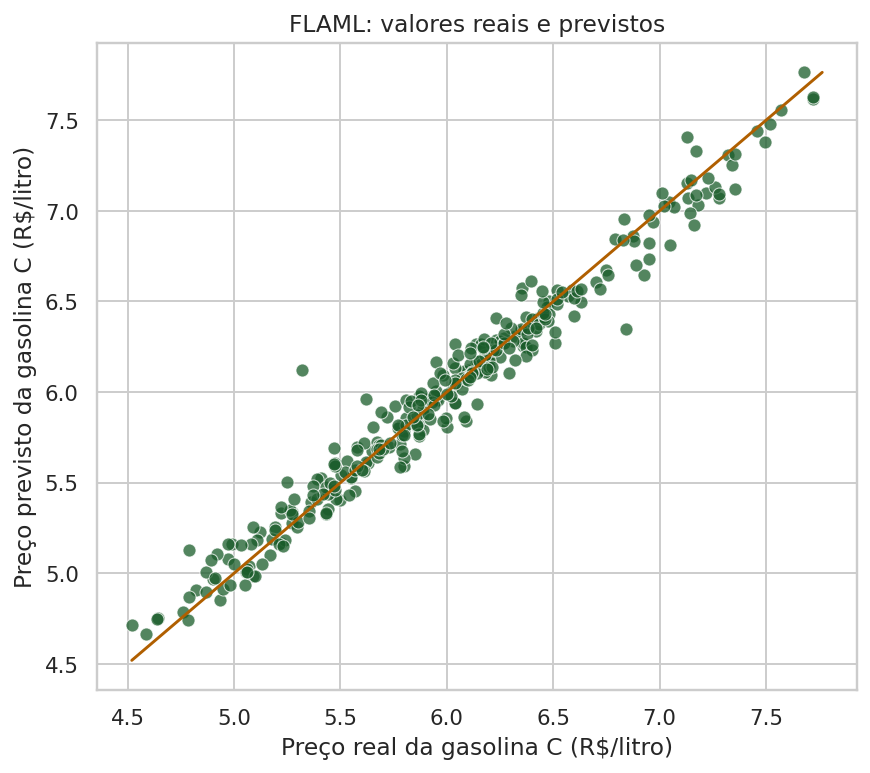
\includegraphics[width=0.75\textwidth]{../../../outputs/figures/flaml_real_vs_previsto.png}
  }{%
    \fbox{\parbox{0.75\textwidth}{Figura \texttt{flaml\_real\_vs\_previsto.png} não encontrada.}}
  }
  \caption{FLAML: comparação entre valores reais e previstos no conjunto de teste.}
  \label{fig:flaml-real-previsto}
\end{figure}

\begin{figure}[H]
  \centering
  \IfFileExists{../../../outputs/figures/flaml_importancia_atributos.png}{%
    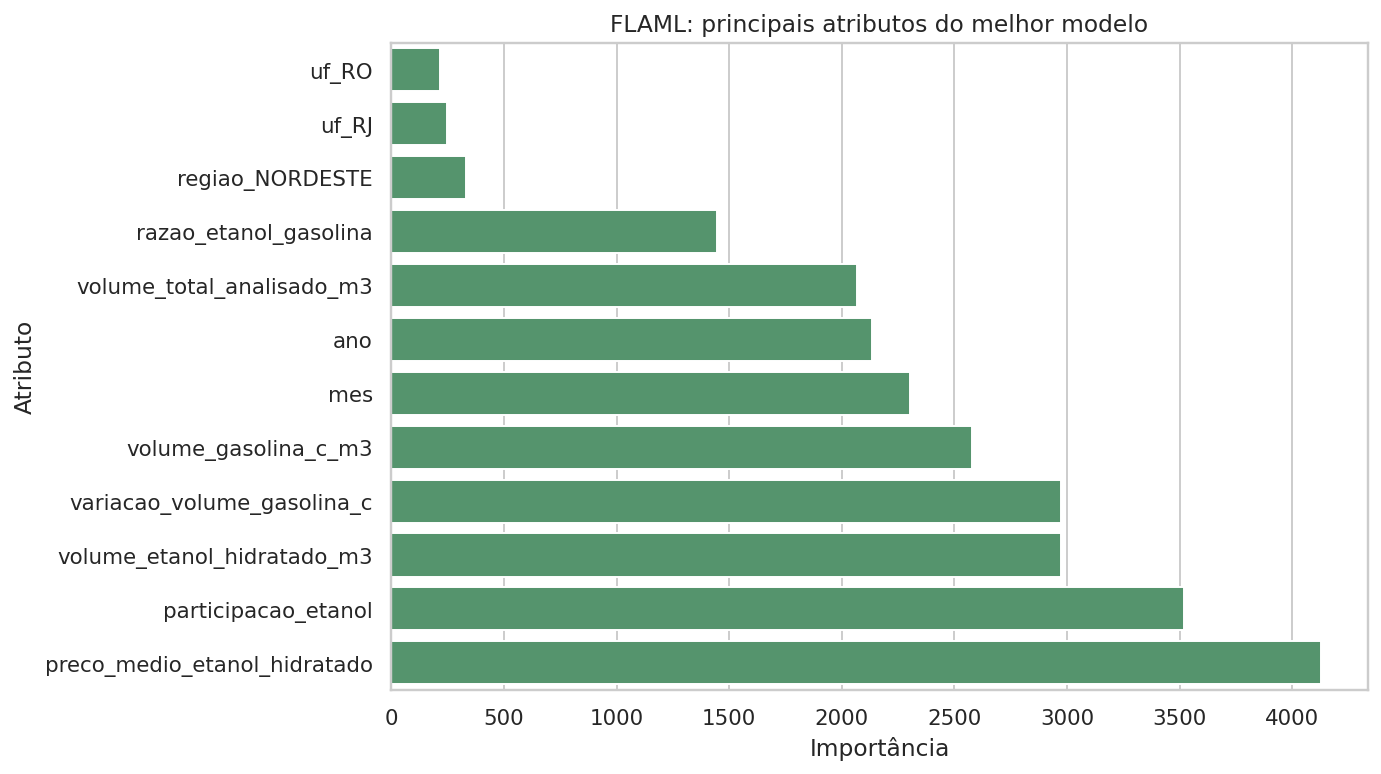
\includegraphics[width=0.84\textwidth]{../../../outputs/figures/flaml_importancia_atributos.png}
  }{%
    \fbox{\parbox{0.75\textwidth}{Figura \texttt{flaml\_importancia\_atributos.png} não encontrada.}}
  }
  \caption{FLAML: principais atributos do melhor modelo selecionado.}
  \label{fig:flaml-importancia}
\end{figure}

\begin{notebox}
\textbf{Síntese da Parte 3:} a FLAML foi fácil de configurar, superou baselines simples
com ampla margem (RMSE reduziu 82,5\% em relação à média do treino), selecionou
\texttt{lgbm} como melhor modelo e gerou métricas, leaderboard, previsões e importância
de atributos dentro de 60 segundos.
\end{notebox}

\newpage

% ==============================================================================
% SEÇÃO 4 - Aplicação da Segunda Ferramenta AutoML (LightAutoML)
% ==============================================================================
\section{Aplicação da Segunda Ferramenta AutoML: LightAutoML}
\label{sec:lightautoml}

\begin{infobox}
\textbf{Objetivo da Parte 4:} aplicar a segunda ferramenta AutoML atribuída à equipe,
documentar o fluxo experimental com os mesmos critérios adotados na Parte 3 e
apresentar os resultados obtidos, preparando a comparação da Parte 5.
\end{infobox}

% ------------------------------------------------------------------------------
\subsection{Nome e breve descrição}
\label{sec:lama-descricao}
% ------------------------------------------------------------------------------

A segunda ferramenta aplicada foi a \textbf{LightAutoML} (LAMA), uma biblioteca de
AutoML desenvolvida pelo Sber AI Lab (anteriormente Sberbank). Diferentemente de
ferramentas que apenas buscam o melhor estimador único, a LightAutoML foi projetada
para construir automaticamente pipelines de múltiplos níveis, incluindo pré-processamento
adaptativo, seleção de features, treinamento de modelos base e combinação por blending.

Sua arquitetura interna organiza o processo em níveis hierárquicos: o primeiro nível
executa vários modelos base (como modelos lineares, LightGBM e redes neurais para
dados tabulares), e os níveis subsequentes combinam as previsões por meio de blending
automático. A ferramenta foi originalmente desenvolvida para lidar com problemas de
grande escala em serviços financeiros, mas funciona bem em datasets tabulares de porte
médio como o utilizado neste experimento.

Entre os diferenciais da LightAutoML em relação à FLAML estão o uso de validação
cruzada interna com mais dobras (5 dobras no experimento), a capacidade de inferência
automática do tipo de cada variável (numérica, categórica, de data) sem necessidade de
pré-processamento manual, e a geração de importância de atributos por meio de gradientes
aproximados.

% ------------------------------------------------------------------------------
\subsection{Instalação e acesso}
\label{sec:lama-instalacao}
% ------------------------------------------------------------------------------

A LightAutoML foi instalada no mesmo ambiente virtual do projeto, ao lado da FLAML,
garantindo que o experimento comparativo fosse realizado no mesmo ambiente de execução.

\begin{tabularx}{\textwidth}{@{}L{4.8cm} Y@{}}
  \toprule
  \thead{Etapa} & \thead{Comando utilizado} \\
  \midrule
  \taltrow Criar ambiente virtual & \texttt{python -m venv .venv} \\
  Ativar ambiente & \texttt{source .venv/bin/activate} \\
  \taltrow Instalar dependências & \texttt{pip install -r requirements.txt} \\
  Instalar LightAutoML & \texttt{pip install lightautoml} \\
  \taltrow Executar experimento & \texttt{python -m src.lightautoml\_analysis} \\
  \bottomrule
\end{tabularx}

\vspace{4mm}

O script reprodutível foi implementado em \texttt{src/lightautoml\_analysis.py}.
Ele carrega o mesmo dataset processado, aplica a mesma divisão treino e teste
definida na Parte 2, treina a LightAutoML com as configurações descritas abaixo e
salva métricas, previsões, importância de atributos e gráficos de apoio.

% ------------------------------------------------------------------------------
\subsection{Preparação para o experimento}
\label{sec:lama-preparacao}
% ------------------------------------------------------------------------------

O arquivo utilizado foi
\texttt{data/processed/dataset\_anp\_pca\_mds\_2021\_2025.csv}, com 1.619 registros.
A mesma divisão da FLAML foi aplicada: 80\% para treino (1.295 registros) e 20\% para
teste (324 registros), com \texttt{random\_state = 42} e estratificação por região.

As mesmas colunas removidas na etapa da FLAML foram excluídas aqui para garantir
comparabilidade:

\begin{itemize}[leftmargin=1.5cm, itemsep=4pt]
  \item \texttt{variacao\_preco\_gasolina\_c}: derivada diretamente da variável-alvo.
  \item \texttt{preco\_relativo\_etanol\_gasolina}: razão que usa o preço da gasolina C no denominador.
  \item \texttt{mes\_ano}: substituída pelas colunas numéricas \texttt{ano} e \texttt{mes}.
  \item \texttt{uf\_nome}: duplica a informação de \texttt{uf}.
\end{itemize}

A LightAutoML realiza o pré-processamento internamente, identificando automaticamente
o tipo de cada coluna. As variáveis categóricas \texttt{uf} e \texttt{regiao} foram
passadas diretamente ao pipeline sem codificação manual prévia, pois a ferramenta
aplica a codificação de forma adaptativa durante o treinamento.

\begin{tabularx}{\textwidth}{@{}L{5.2cm} Y@{}}
  \toprule
  \thead{Configuração} & \thead{Valor} \\
  \midrule
  \taltrow Tipo de problema & Regressão (\texttt{reg}) \\
  Variável-alvo & \texttt{preco\_medio\_gasolina\_c} \\
  \taltrow Métrica interna & MSE (minimização) \\
  Métrica principal de avaliação & RMSE \\
  \taltrow Divisão dos dados & 80\% treino e 20\% teste \\
  Validação cruzada interna & 5 dobras (\texttt{cv = 5}) \\
  \taltrow Semente aleatória & 42 \\
  Orçamento de tempo & 120 segundos \\
  \taltrow Limite de CPUs & 4 \\
  \bottomrule
\end{tabularx}

% ------------------------------------------------------------------------------
\subsection{Principais comandos e etapas utilizadas}
\label{sec:lama-etapas}
% ------------------------------------------------------------------------------

As principais etapas executadas no script foram:

\begin{enumerate}[leftmargin=1.5cm, itemsep=4pt]
  \item Carregamento do dataset processado da ANP.
  \item Separação da variável-alvo \texttt{preco\_medio\_gasolina\_c}.
  \item Remoção de colunas que poderiam causar vazamento de dados ou duplicidade.
  \item Divisão treino e teste com estratificação por região.
  \item Definição da tarefa de regressão com a classe \texttt{Task("reg", metric="mse")}.
  \item Instanciação do \texttt{TabularAutoML} com orçamento de 120 segundos e 5 dobras de validação cruzada.
  \item Treinamento automático via \texttt{fit\_predict()}, que executa internamente a construção do pipeline completo.
  \item Predição no conjunto de teste via \texttt{predict()}.
  \item Cálculo de RMSE, MAE, R² e MAPE no conjunto de teste.
  \item Extração da importância de atributos via \texttt{get\_feature\_scores("fast")}.
  \item Geração de métricas, previsões, análise de erros por região e gráficos.
\end{enumerate}

% ------------------------------------------------------------------------------
\subsection{Modelos testados automaticamente}
\label{sec:lama-modelos}
% ------------------------------------------------------------------------------

A LightAutoML constrói automaticamente um pipeline de múltiplos níveis, sem expor
diretamente um leaderboard comparativo de estimadores individuais como a FLAML. No
nível base, o pipeline tabular padrão (\texttt{TabularAutoML}) inclui:

\begin{itemize}[leftmargin=1.5cm, itemsep=4pt]
  \item \textbf{Modelos lineares regularizados:} utilizados como modelos base de nível 0, com regularização L1 ou L2 definida automaticamente.
  \item \textbf{LightGBM:} gradient boosting baseado em LightGBM, com hiperparâmetros ajustados por busca interna.
  \item \textbf{Combinação por blending:} no segundo nível, as previsões dos modelos base são combinadas por um modelo de blending treinado nas previsões de validação cruzada.
\end{itemize}

O pipeline final executado dentro do orçamento de 120 segundos incluiu os modelos base
lineares e o LightGBM, combinados por blending automático. As previsões fora da amostra
(out-of-fold) geradas durante a validação cruzada foram usadas para treinar o blender.

% ------------------------------------------------------------------------------
\subsection{Melhor modelo e métricas obtidas}
\label{sec:lama-resultados}
% ------------------------------------------------------------------------------

O pipeline final gerado pela LightAutoML obteve os seguintes resultados no conjunto
de teste, que não foi utilizado em nenhuma etapa do treinamento:

\begin{center}
\begin{tabularx}{0.9\textwidth}{@{}L{4.5cm} C{4cm} Y@{}}
  \toprule
  \thead{Métrica} & \thead{Valor} & \thead{Interpretação} \\
  \midrule
  \taltrow RMSE & 0,1134 & Erro médio quadrático em R\$/litro. \\
  MAE & 0,0888 & Erro absoluto médio de aproximadamente nove centavos por litro. \\
  \taltrow R² & 0,9701 & O modelo explicou 97,01\% da variação observada no teste. \\
  MAPE & 1,4942\% & Erro percentual médio para o recorte testado. \\
  \taltrow Tempo de execução & 73,94 segundos & Dentro do orçamento definido de 120s. \\
  \bottomrule
\end{tabularx}
\end{center}

\begin{figure}[H]
  \centering
  \IfFileExists{../../../outputs/figures/lightautoml_real_vs_previsto.png}{%
    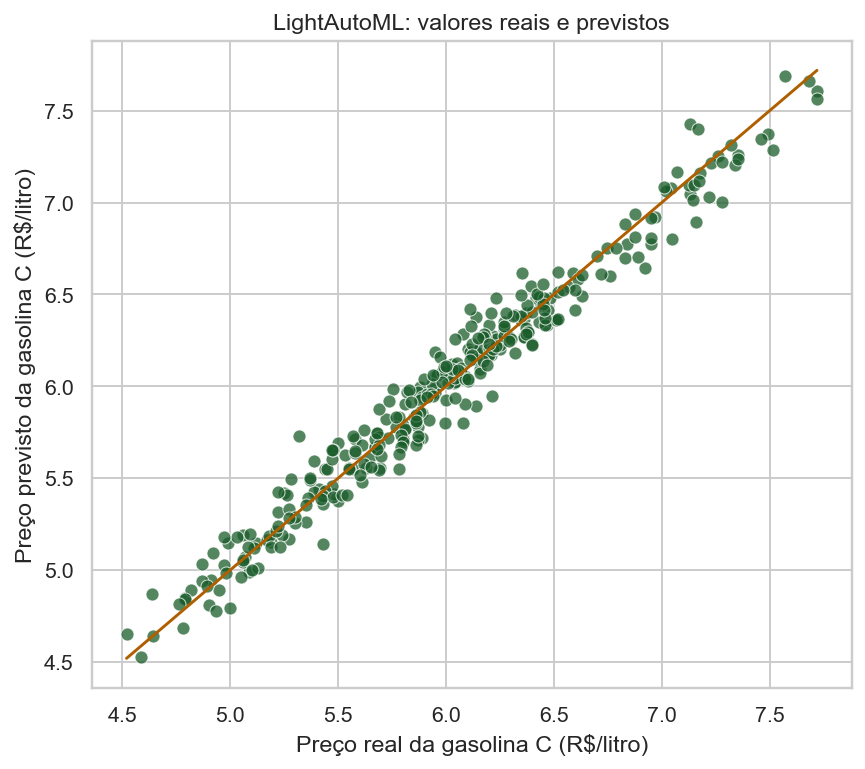
\includegraphics[width=0.75\textwidth]{../../../outputs/figures/lightautoml_real_vs_previsto.png}
  }{%
    \fbox{\parbox{0.75\textwidth}{Figura \texttt{lightautoml\_real\_vs\_previsto.png} não encontrada.}}
  }
  \caption{LightAutoML: comparação entre valores reais e previstos no conjunto de teste.}
  \label{fig:lama-real-previsto}
\end{figure}

\begin{infobox}
\textbf{Leitura dos resultados:} o RMSE de 0,1134 e o R² de 0,9701 indicam que o
pipeline construído automaticamente pela LightAutoML capturou com boa fidelidade a
estrutura dos preços de combustíveis no período analisado. O erro absoluto médio de
aproximadamente R\$ 0,09 por litro é baixo para o contexto do problema.
\end{infobox}

% ------------------------------------------------------------------------------
\subsection{Recursos gerados pela ferramenta}
\label{sec:lama-recursos}
% ------------------------------------------------------------------------------

O experimento gerou os seguintes artefatos no projeto:

\begin{tabularx}{\textwidth}{@{}L{6.5cm} Y@{}}
  \toprule
  \thead{Arquivo} & \thead{Conteúdo} \\
  \midrule
  \taltrow \path{outputs/tables/lightautoml_metricas.csv} & Métricas finais no conjunto de teste, tempo de execução e configuração geral. \\
  \path{outputs/tables/lightautoml_importancia_atributos.csv} & Importância dos atributos calculada pelo método \texttt{get\_feature\_scores("fast")}. \\
  \taltrow \path{outputs/tables/lightautoml_previsoes_teste.csv} & Valores reais, previsões e erros no conjunto de teste. \\
  \path{outputs/tables/lightautoml_analise_erros_regiao.csv} & Resumo dos erros médios por região no conjunto de teste. \\
  \taltrow \path{outputs/tables/lightautoml_resumo_erros.csv} & Estatísticas resumidas da distribuição dos resíduos. \\
  \path{outputs/figures/lightautoml_real_vs_previsto.png} & Gráfico de valores reais contra valores previstos. \\
  \taltrow \path{outputs/figures/lightautoml_importancia_atributos.png} & Gráfico dos principais atributos do pipeline. \\
  \path{outputs/figures/lightautoml_hist_erro_absoluto.png} & Distribuição dos erros absolutos. \\
  \taltrow \path{outputs/figures/lightautoml_mae_por_regiao.png} & Erro absoluto médio por região. \\
  \bottomrule
\end{tabularx}

% ------------------------------------------------------------------------------
\subsection{Importância dos atributos}
\label{sec:lama-importancia}
% ------------------------------------------------------------------------------

A importância dos atributos foi obtida via \texttt{get\_feature\_scores("fast")},
que retorna a contribuição de cada variável para o pipeline treinado. Os dez atributos
mais importantes foram:

\begin{center}
\begin{tabularx}{0.88\textwidth}{@{}C{0.8cm} L{6.5cm} C{4cm}@{}}
  \toprule
  \thead{Rank} & \thead{Atributo} & \thead{Importância} \\
  \midrule
  \taltrow 1 & \texttt{preco\_medio\_etanol\_hidratado} & 9.642,29 \\
  2 & \texttt{ano} & 4.613,17 \\
  \taltrow 3 & \texttt{participacao\_etanol} & 2.963,76 \\
  4 & \texttt{mes} & 865,96 \\
  \taltrow 5 & \texttt{volume\_gasolina\_c\_m3} & 550,67 \\
  6 & \texttt{razao\_etanol\_gasolina} & 529,31 \\
  \taltrow 7 & \texttt{volume\_etanol\_hidratado\_m3} & 481,90 \\
  8 & \texttt{volume\_total\_analisado\_m3} & 288,75 \\
  \taltrow 9 & \texttt{variacao\_volume\_gasolina\_c} & 120,22 \\
  10 & \texttt{uf} & 0,00 \\
  \bottomrule
\end{tabularx}
\end{center}

\vspace{4mm}

O atributo mais importante foi o preço do etanol hidratado, o que é esperado dada a
forte correlação de mercado entre os dois combustíveis. Em segundo lugar, o atributo
\texttt{ano} capturou a tendência de alta observada no período de 2021 a 2025. A
participação do etanol e o mês de referência completam os quatro atributos de maior
peso, refletindo a sazonalidade dos preços e a dinâmica de substituição entre
combustíveis.

Um resultado interessante é que as variáveis categóricas \texttt{uf} e \texttt{regiao}
obtiveram importância zero no método rápido de cálculo. Isso pode indicar que, após
o controle das variáveis contínuas de preço, volume e tempo, a variação regional já
estava capturada indiretamente pelos demais atributos. Esse comportamento difere
da FLAML, em que a codificação one-hot das categorias regionais contribuiu de forma
mais explícita para o modelo.

\begin{figure}[H]
  \centering
  \IfFileExists{../../../outputs/figures/lightautoml_importancia_atributos.png}{%
    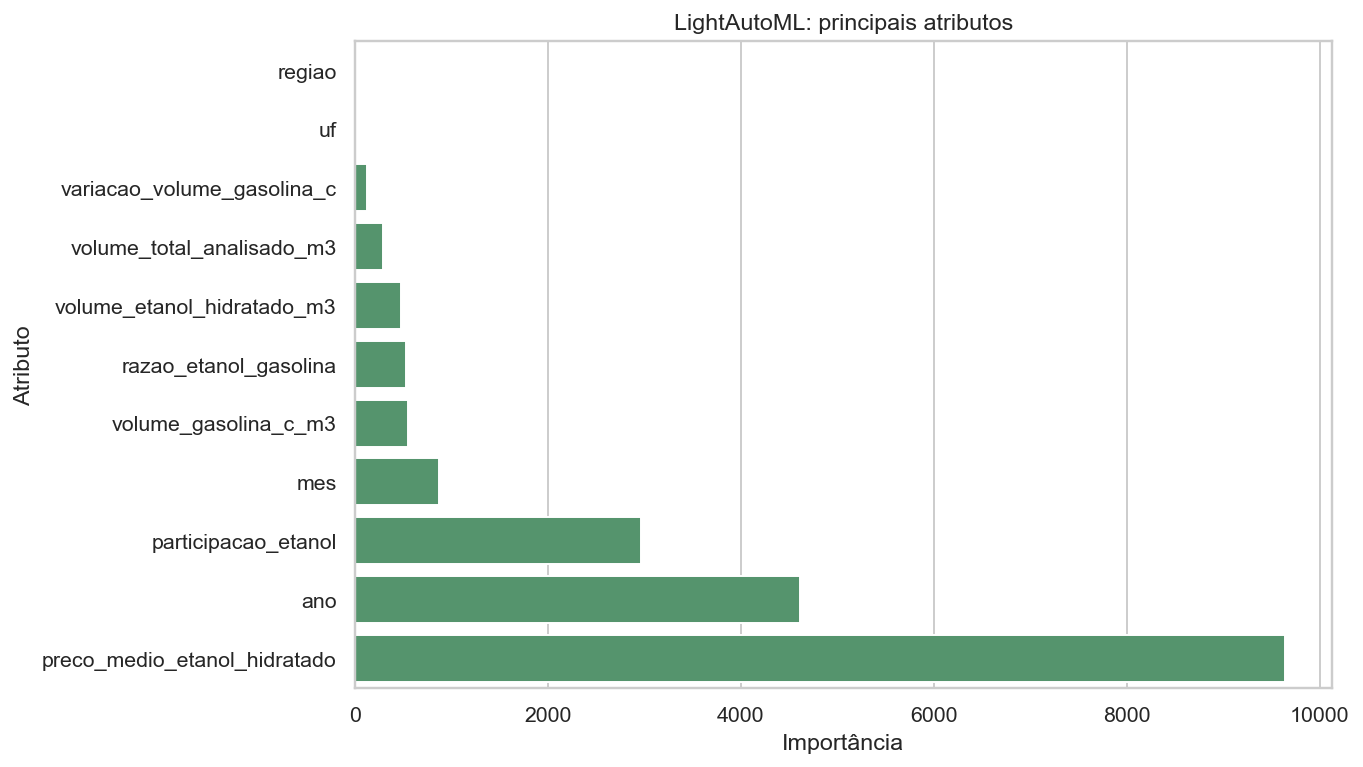
\includegraphics[width=0.84\textwidth]{../../../outputs/figures/lightautoml_importancia_atributos.png}
  }{%
    \fbox{\parbox{0.75\textwidth}{Figura \texttt{lightautoml\_importancia\_atributos.png} não encontrada.}}
  }
  \caption{LightAutoML: importância dos atributos no pipeline treinado.}
  \label{fig:lama-importancia}
\end{figure}

% ------------------------------------------------------------------------------
\subsection{Análise dos erros no conjunto de teste}
\label{sec:lama-erros}
% ------------------------------------------------------------------------------

A distribuição dos resíduos da LightAutoML no conjunto de teste apresentou as
seguintes características:

\begin{table}[H]
\centering
\small
\setlength{\tabcolsep}{5pt}
\begin{tabularx}{0.78\textwidth}{@{}Y C{2.35cm}@{}}
  \toprule
  \thead{Resumo do erro} & \thead{Valor} \\
  \midrule
  \taltrow Mediana do erro absoluto & 0,0718 \\
  75\% dos erros absolutos & 0,1276 \\
  \taltrow 90\% dos erros absolutos & 0,1916 \\
  95\% dos erros absolutos & 0,2277 \\
  Máximo erro absoluto & 0,4180 \\
  \taltrow Desvio-padrão do erro assinado & 0,1135 \\
  Erro médio assinado & -0,0028 \\
  \bottomrule
\end{tabularx}
\caption{Resumo da distribuição dos resíduos da LightAutoML no conjunto de teste.}
\label{tab:lama-resumo-erros}
\end{table}

A maior parte das previsões ficou com erro absoluto abaixo de R\$ 0,13 por litro
(percentil 75). O erro médio assinado foi praticamente nulo (-0,0028), o que indica
ausência de viés sistemático relevante. O maior erro absoluto observado foi de R\$ 0,42,
consideravelmente menor do que o máximo da FLAML (R\$ 0,80).

Em nível regional, os erros ficaram distribuídos da seguinte forma:

\begin{table}[H]
\centering
\small
\setlength{\tabcolsep}{4.5pt}
\begin{tabularx}{0.92\textwidth}{@{}Y C{1.45cm} C{1.45cm} C{1.6cm} C{1.6cm}@{}}
  \toprule
  \thead{Região} & \thead{MAE} & \thead{RMSE} & \thead{Erro médio} & \thead{MAPE} \\
  \midrule
  \taltrow CENTRO OESTE & 0,0760 & 0,0968 & 0,0120 & 1,2865\% \\
  SUDESTE & 0,0848 & 0,1127 & -0,0264 & 1,4508\% \\
  \taltrow NORDESTE & 0,0888 & 0,1140 & -0,0052 & 1,4807\% \\
  NORTE & 0,0917 & 0,1165 & 0,0186 & 1,5195\% \\
  \taltrow SUL & 0,1048 & 0,1251 & -0,0334 & 1,8105\% \\
  \bottomrule
\end{tabularx}
\caption{Erro médio da LightAutoML por região no conjunto de teste.}
\label{tab:lama-erro-regiao}
\end{table}

O Centro-Oeste apresentou o menor erro médio, enquanto o Sul manteve o maior MAE entre
as regiões, o mesmo padrão observado na FLAML. Isso sugere que o Sul tem características
específicas de preços e volumes que tornam a previsão mais desafiadora independentemente
da ferramenta utilizada.

\begin{figure}[H]
  \centering
  \IfFileExists{../../../outputs/figures/lightautoml_mae_por_regiao.png}{%
    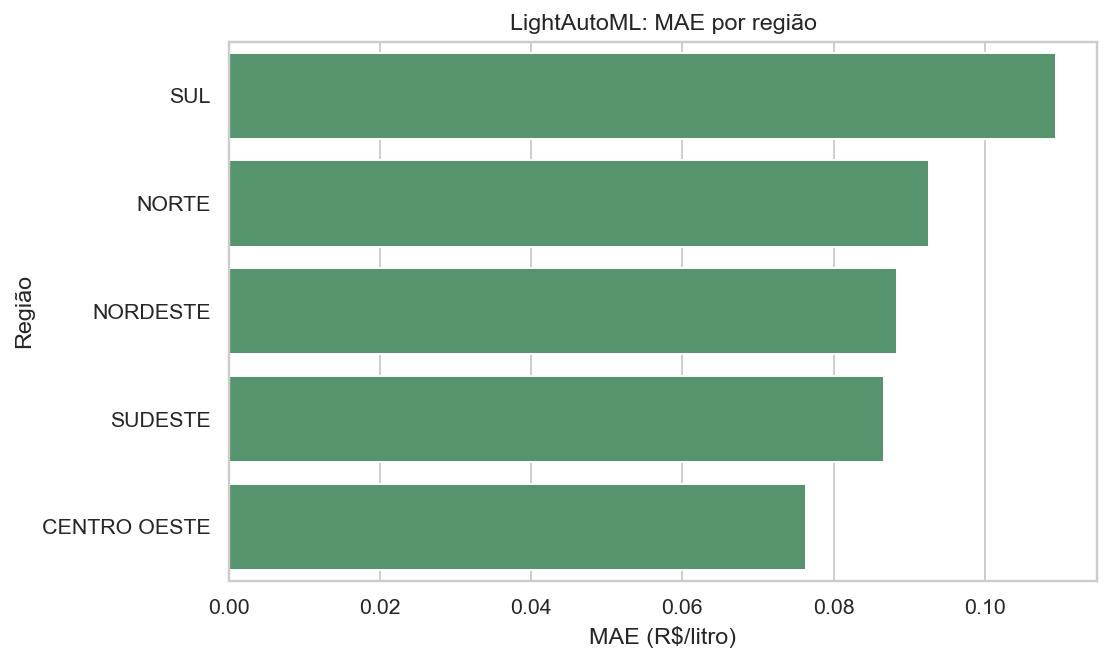
\includegraphics[width=0.76\textwidth]{../../../outputs/figures/lightautoml_mae_por_regiao.png}
  }{%
    \fbox{\parbox{0.75\textwidth}{Figura \texttt{lightautoml\_mae\_por\_regiao.png} não encontrada.}}
  }
  \caption{LightAutoML: erro absoluto médio por região.}
  \label{fig:lama-mae-regiao}
\end{figure}

\begin{figure}[H]
  \centering
  \IfFileExists{../../../outputs/figures/lightautoml_hist_erro_absoluto.png}{%
    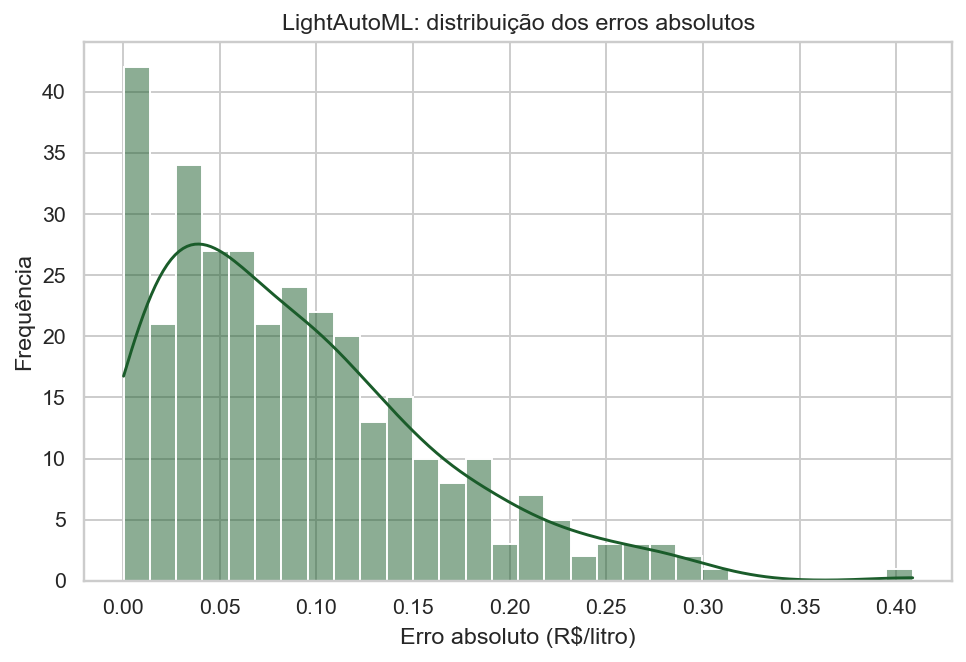
\includegraphics[width=0.76\textwidth]{../../../outputs/figures/lightautoml_hist_erro_absoluto.png}
  }{%
    \fbox{\parbox{0.75\textwidth}{Figura \texttt{lightautoml\_hist\_erro\_absoluto.png} não encontrada.}}
  }
  \caption{LightAutoML: distribuição dos erros absolutos no conjunto de teste.}
  \label{fig:lama-hist-erro}
\end{figure}

% ------------------------------------------------------------------------------
\subsection{Validade experimental da Parte 4}
\label{sec:lama-validade}
% ------------------------------------------------------------------------------

Para que a comparação com a FLAML fosse justa, a aplicação da LightAutoML seguiu
os mesmos cuidados metodológicos da primeira ferramenta. O conjunto de teste foi
mantido isolado até a etapa final de avaliação, a estratificação por região foi
preservada e as colunas derivadas diretamente da variável-alvo foram removidas antes
do treinamento.

\begin{tabularx}{\textwidth}{@{}L{5.2cm} Y@{}}
  \toprule
  \thead{Critério de controle} & \thead{Como foi aplicado} \\
  \midrule
  \taltrow Mesma base de dados & Uso do arquivo tratado \texttt{dataset\_anp\_pca\_mds\_2021\_2025.csv}. \\
  Mesma divisão experimental & 80\% treino e 20\% teste, com \texttt{random\_state = 42} e estratificação por região. \\
  \taltrow Mesma variável-alvo & Previsão de \texttt{preco\_medio\_gasolina\_c}. \\
  Mesmo controle de vazamento & Remoção de \texttt{variacao\_preco\_gasolina\_c} e \texttt{preco\_relativo\_etanol\_gasolina}. \\
  \taltrow Mesma métrica central & RMSE calculado no conjunto de teste. \\
  Reprodutibilidade & Scripts, tabelas e figuras salvos no repositório para auditoria dos resultados. \\
  \bottomrule
\end{tabularx}

Mesmo com esses controles, a comparação deve ser interpretada como um experimento
didático e exploratório. O orçamento de tempo não foi idêntico porque a LightAutoML
precisou de maior folga para completar seu pipeline multinível, enquanto a FLAML foi
avaliada com orçamento menor e estimadores explicitamente limitados.

% ------------------------------------------------------------------------------
\subsection{Síntese da aplicação da LightAutoML}
\label{sec:lama-sintese}
% ------------------------------------------------------------------------------

A LightAutoML apresentou desempenho muito próximo ao da FLAML, com RMSE de 0,1134
e R² de 0,9701 no conjunto de teste. O pipeline de múltiplos níveis construído
automaticamente conseguiu capturar a estrutura dos preços com fidelidade elevada,
mantendo erro médio abaixo de R\$ 0,09 por litro.

A configuração exigiu mais etapas de instalação e compreensão da API, mas a ferramenta
assumiu automaticamente a responsabilidade pelo pré-processamento, tipo das variáveis
e construção do pipeline completo. O tempo de execução foi maior que o da FLAML
(73,94s contra 60,78s), mas ainda dentro de um orçamento aceitável.

\begin{notebox}
\textbf{Síntese da Parte 4:} a LightAutoML construiu automaticamente um pipeline
de múltiplos níveis com LightGBM e blending, obteve RMSE = 0,1134 e R² = 0,9701
no conjunto de teste, gerou importância de atributos e análise de erros por região,
e executou dentro do orçamento de 120 segundos. O atributo mais importante foi o
preço do etanol hidratado, seguido pelo ano e pela participação do etanol.
\end{notebox}

\newpage

% ==============================================================================
% SEÇÃO 5 - Reflexão e Comparação
% ==============================================================================
\section{Reflexão e Comparação das Ferramentas}
\label{sec:reflexao}

\begin{infobox}
\textbf{Objetivo da Parte 5:} responder às questões de reflexão propostas na atividade
com base na experiência prática da equipe na aplicação de FLAML e LightAutoML ao
dataset de combustíveis ANP.
\end{infobox}

% ------------------------------------------------------------------------------
\subsection{Comparativo de desempenho}
\label{sec:comparativo-desempenho}
% ------------------------------------------------------------------------------

Antes de responder às questões de reflexão, apresenta-se o comparativo consolidado
das métricas obtidas pelas duas ferramentas no mesmo conjunto de teste:

\begin{table}[H]
\centering
\small
\setlength{\tabcolsep}{4.5pt}
\begin{tabularx}{\textwidth}{@{}Y C{2cm} C{2cm} C{2cm} C{2cm} C{2.4cm}@{}}
  \toprule
  \thead{Ferramenta} & \thead{RMSE} & \thead{MAE} & \thead{R²} & \thead{MAPE} & \thead{Tempo (s)} \\
  \midrule
  \taltrow FLAML (\texttt{lgbm}) & 0,1148 & 0,0819 & 0,9693 & 1,3841\% & 60,78 \\
  LightAutoML & 0,1134 & 0,0888 & 0,9701 & 1,4942\% & 73,94 \\
  \bottomrule
\end{tabularx}
\caption{Comparativo de desempenho entre FLAML e LightAutoML no conjunto de teste.}
\label{tab:comparativo}
\end{table}

A diferença entre as ferramentas foi pequena em todas as métricas, com vantagem
parcial para a LightAutoML em RMSE e R² e para a FLAML em MAE e MAPE. Isso indica
que ambas chegaram a soluções de qualidade equivalente para este problema.

% ------------------------------------------------------------------------------
\subsection{Qual ferramenta foi mais fácil de usar?}
\label{sec:facilidade}
% ------------------------------------------------------------------------------

A \textbf{FLAML} foi consideravelmente mais fácil de usar. Sua API é direta: basta
instanciar o \texttt{AutoML()}, definir o tipo de tarefa e o orçamento de tempo e
chamar \texttt{fit()}. O leaderboard comparativo de estimadores fica acessível de
forma imediata, o que facilita a compreensão do que aconteceu durante o treinamento.

A LightAutoML exige um nível de compreensão maior da arquitetura da ferramenta. A
definição da tarefa usa uma classe própria (\texttt{Task}), o método de treinamento
é \texttt{fit\_predict()} em vez do padrão \texttt{fit()}, e a extração de importância
de atributos requer um passo adicional com \texttt{get\_feature\_scores()}. Além disso,
o pipeline interno da LightAutoML não expõe diretamente os modelos avaliados em cada
nível, o que dificulta a inspeção do processo por usuários iniciantes.

Por fim, a instalação da LightAutoML gerou avisos relacionados a pacotes opcionais
de processamento de linguagem natural não instalados (como \texttt{fasttext} e
\texttt{transformers}), o que pode confundir usuários sem experiência.

% ------------------------------------------------------------------------------
\subsection{Qual ferramenta apresentou melhor desempenho?}
\label{sec:melhor-desempenho}
% ------------------------------------------------------------------------------

O desempenho foi muito próximo. A \textbf{LightAutoML} teve leve vantagem em RMSE
(0,1134 contra 0,1148) e em R² (0,9701 contra 0,9693). Por outro lado, a
\textbf{FLAML} teve melhor MAE (0,0819 contra 0,0888) e melhor MAPE (1,3841\%
contra 1,4942\%). Em termos práticos, a diferença de RMSE foi de apenas 0,0014,
o que equivale a menos de R\$ 0,002 por litro.

Considerando a métrica principal adotada na atividade (RMSE), a LightAutoML foi
ligeiramente superior. Entretanto, as diferenças observadas são tão pequenas que
qualquer variação no conjunto de treino ou nas sementes aleatórias poderia inverter
esse resultado. A conclusão mais robusta é que \textbf{as duas ferramentas chegaram
a soluções de desempenho equivalente para este problema}.

% ------------------------------------------------------------------------------
\subsection{A ferramenta com melhor desempenho também foi a mais fácil de usar?}
\label{sec:facilidade-vs-desempenho}
% ------------------------------------------------------------------------------

\textbf{Não.} A LightAutoML obteve o melhor RMSE, mas a FLAML foi a ferramenta mais
fácil de configurar e usar. Esse resultado ilustra um dilema frequente em AutoML:
ferramentas com pipelines mais sofisticados e potencialmente mais poderosos tendem
a ter curvas de aprendizado mais íngremes. Para este problema específico, a diferença
de desempenho não foi suficientemente grande para justificar a complexidade adicional
da LightAutoML, especialmente em um contexto de uso inicial ou prototipação rápida.

% ------------------------------------------------------------------------------
\subsection{Alguma ferramenta gerou explicações sobre os resultados?}
\label{sec:explicacoes}
% ------------------------------------------------------------------------------

Ambas as ferramentas geraram alguma forma de explicabilidade, mas com diferenças:

\begin{itemize}[leftmargin=1.5cm, itemsep=4pt]
  \item \textbf{FLAML:} forneceu a importância de atributos baseada no ganho do LightGBM, além de um leaderboard com os estimadores avaliados e os hiperparâmetros do melhor modelo. Essas informações são relativamente fáceis de interpretar.
  \item \textbf{LightAutoML:} forneceu importância de atributos via gradientes aproximados (\texttt{get\_feature\_scores("fast")}), mas não expôs diretamente o processo de seleção dos modelos internos nem os hiperparâmetros ajustados. A ausência de um leaderboard comparativo reduz a transparência do processo.
\end{itemize}

Nenhuma das duas ferramentas gerou explicações no nível de SHAP ou LIME de forma
automática, o que seria necessário para interpretar previsões individuais. A geração
de explicações em nível de instância continuou sendo uma etapa humana.

% ------------------------------------------------------------------------------
\subsection{O AutoML ajudou a reduzir o tempo de desenvolvimento?}
\label{sec:tempo}
% ------------------------------------------------------------------------------

\textbf{Sim, de forma significativa.} Sem AutoML, a equipe teria que:

\begin{enumerate}[leftmargin=1.5cm, itemsep=4pt]
  \item Selecionar manualmente os algoritmos candidatos.
  \item Definir grades de hiperparâmetros para cada algoritmo.
  \item Implementar a busca por validação cruzada.
  \item Comparar os resultados e selecionar o melhor modelo.
  \item Repetir o processo iterativamente até atingir um desempenho satisfatório.
\end{enumerate}

Com a FLAML, esse processo foi reduzido a menos de 61 segundos de execução. Com a
LightAutoML, a menos de 74 segundos. O esforço humano se concentrou na preparação
dos dados, na definição do problema e na interpretação dos resultados.

% ------------------------------------------------------------------------------
\subsection{Quais decisões ainda precisaram ser tomadas pela equipe?}
\label{sec:decisoes-humanas}
% ------------------------------------------------------------------------------

Mesmo com o uso de AutoML, a equipe precisou tomar as seguintes decisões:

\begin{itemize}[leftmargin=1.5cm, itemsep=4pt]
  \item \textbf{Escolha do dataset:} selecionar o dataset de combustíveis ANP como base para os experimentos.
  \item \textbf{Definição da variável-alvo:} escolher \texttt{preco\_medio\_gasolina\_c} como alvo do problema de regressão.
  \item \textbf{Remoção de colunas com vazamento de dados:} identificar quais atributos deveriam ser excluídos para evitar contaminação do modelo.
  \item \textbf{Definição da métrica principal:} optar por RMSE como métrica central de comparação.
  \item \textbf{Orçamento de tempo:} definir 60 segundos para a FLAML e 120 segundos para a LightAutoML.
  \item \textbf{Interpretação dos resultados:} analisar a importância dos atributos no contexto do mercado de combustíveis.
  \item \textbf{Análise dos erros por região:} avaliar se o desempenho era uniforme entre as cinco regiões brasileiras.
\end{itemize}

% ------------------------------------------------------------------------------
\subsection{Quais problemas poderiam ocorrer sem compreensão de Ciência de Dados?}
\label{sec:riscos-sem-conhecimento}
% ------------------------------------------------------------------------------

O uso de AutoML sem compreensão dos fundamentos de Ciência de Dados pode gerar
problemas sérios:

\begin{itemize}[leftmargin=1.5cm, itemsep=4pt]
  \item \textbf{Vazamento de dados:} sem remover as colunas derivadas do alvo, o modelo teria aprendido a usar informações que não estariam disponíveis em produção, gerando métricas artificialmente otimistas.
  \item \textbf{Escolha inadequada da métrica:} usar acurácia em um problema de regressão ou RMSE quando o negócio exige minimizar erros grandes seria um equívoco que o AutoML não detecta automaticamente.
  \item \textbf{Interpretação incorreta dos resultados:} um R² de 0,97 pode parecer excelente, mas um usuário sem conhecimento não saberia avaliar se o modelo seria generalizável para dados futuros ou se estava apenas memorizando padrões históricos.
  \item \textbf{Overfitting não detectado:} sem compreender a divisão treino-teste e validação cruzada, o usuário poderia aceitar métricas calculadas sobre dados de treino como resultado final.
  \item \textbf{Implantação irresponsável:} um modelo de previsão de preços aplicado sem monitoramento e sem entendimento das suas limitações poderia gerar decisões prejudiciais em contextos reais.
\end{itemize}

% ------------------------------------------------------------------------------
\subsection{Em que situações o AutoML pode ser útil em projetos reais?}
\label{sec:util}
% ------------------------------------------------------------------------------

O AutoML é especialmente útil quando:

\begin{itemize}[leftmargin=1.5cm, itemsep=4pt]
  \item \textbf{Prototipação rápida:} há necessidade de avaliar rapidamente a viabilidade de um problema de ML antes de investir em soluções mais elaboradas.
  \item \textbf{Benchmark de baseline:} o objetivo é estabelecer um ponto de referência inicial para comparar com soluções personalizadas.
  \item \textbf{Dados tabulares bem estruturados:} o problema envolve datasets com estrutura clara, sem necessidade de engenharia de features altamente especializada.
  \item \textbf{Equipes com diferentes perfis técnicos:} quando analistas e especialistas de domínio precisam construir modelos sem depender exclusivamente de cientistas de dados.
  \item \textbf{Projetos com restrição de tempo:} quando há prazos curtos e a qualidade do baseline automático é suficiente para o propósito.
\end{itemize}

% ------------------------------------------------------------------------------
\subsection{Em que situações o AutoML pode não ser adequado?}
\label{sec:nao-adequado}
% ------------------------------------------------------------------------------

O AutoML pode ser insuficiente ou inadequado quando:

\begin{itemize}[leftmargin=1.5cm, itemsep=4pt]
  \item \textbf{Dados não estruturados:} problemas com imagens, texto livre, áudio ou séries temporais complexas geralmente exigem arquiteturas específicas que as ferramentas AutoML padrão não cobrem bem.
  \item \textbf{Requisitos de interpretabilidade regulatória:} setores como saúde, crédito e seguros exigem que os modelos sejam explicáveis de forma auditável, o que ensembles complexos gerados por AutoML dificilmente atendem.
  \item \textbf{Domínios com lógica de negócio específica:} quando as features mais relevantes dependem de conhecimento profundo do domínio para serem construídas, o AutoML pode não explorar adequadamente o espaço de hipóteses relevantes.
  \item \textbf{Datasets muito grandes:} o custo computacional da busca automática em datasets com dezenas de milhões de registros pode ser proibitivo sem infraestrutura adequada.
  \item \textbf{Problemas de produção críticos:} quando o modelo precisa ser validado, monitorado e explicado em nível de instância para conformidade regulatória.
\end{itemize}

% ------------------------------------------------------------------------------
\subsection{Qual ferramenta a equipe recomendaria para iniciantes?}
\label{sec:recomendacao}
% ------------------------------------------------------------------------------

A equipe recomenda a \textbf{FLAML} para iniciantes. As razões são:

\begin{enumerate}[leftmargin=1.5cm, itemsep=4pt]
  \item \textbf{API intuitiva e próxima ao padrão scikit-learn:} a interface da FLAML é familiar para quem já conhece sklearn, facilitando a curva de aprendizado.
  \item \textbf{Transparência do processo:} o leaderboard comparativo permite que o usuário entenda quais algoritmos foram avaliados e por que o melhor foi selecionado, algo pedagógico para quem está aprendendo.
  \item \textbf{Instalação simples:} \texttt{pip install flaml} sem dependências conflitantes ou avisos de pacotes opcionais.
  \item \textbf{Desempenho competitivo:} para datasets tabulares de porte médio, a diferença de desempenho em relação a ferramentas mais complexas é pequena, como demonstrado neste experimento.
  \item \textbf{Documentação acessível:} a documentação oficial da FLAML é clara e possui exemplos didáticos.
\end{enumerate}

A LightAutoML é recomendada para usuários com maior experiência que desejam pipelines
mais sofisticados, especialmente em problemas com datasets financeiros ou corporativos
de maior complexidade.

\begin{infobox}
\textbf{Síntese da Parte 5:} as duas ferramentas produziram resultados equivalentes
para este problema, com RMSE de 0,1148 (FLAML) e 0,1134 (LightAutoML). A FLAML foi
mais fácil de usar, mais transparente e igualmente competitiva. A LightAutoML teve
leve vantagem em RMSE e R², mas maior complexidade de uso. Para iniciantes, a equipe
recomenda a FLAML. Para projetos com maior exigência de sofisticação e pipeline
automatizado de múltiplos níveis, a LightAutoML é uma opção mais robusta.
\end{infobox}

\subsection{Encaminhamento final}
\label{sec:encaminhamento-final}

Como encaminhamento, a equipe entende que o AutoML cumpriu bem o papel de acelerar a
construção de modelos fortes para dados tabulares. O experimento também mostrou que
comparar ferramentas apenas pela menor métrica pode ser insuficiente: facilidade de
uso, interpretabilidade, custo computacional, documentação e clareza do pipeline são
critérios tão importantes quanto pequenas diferenças numéricas.

Em um projeto real, o próximo passo seria validar os modelos em uma janela temporal
posterior, acompanhar a estabilidade dos erros por UF e região, e produzir explicações
locais das previsões para casos de maior impacto. Assim, o AutoML seria usado como
base técnica inicial, mas a decisão final continuaria apoiada por validação humana e
conhecimento do domínio de combustíveis.

% ==============================================================================
% Referências
% ==============================================================================
\newpage
\section*{Referências}
\addcontentsline{toc}{section}{Referências}

\begin{itemize}[leftmargin=1.5cm, itemsep=4pt]
  \item ANP. \textit{Série histórica do levantamento de preços de combustíveis}. Agência Nacional do Petróleo, Gás Natural e Biocombustíveis. Disponível em: \url{https://www.gov.br/anp/pt-br/centrais-de-conteudo/dados-abertos/serie-historica-do-levantamento-de-precos}
  \item ANP. \textit{Vendas de derivados de petróleo e biocombustíveis por UF}. Disponível em: \url{https://www.gov.br/anp/pt-br/centrais-de-conteudo/dados-abertos/vendas-de-derivados-de-petroleo-e-biocombustiveis}
  \item HUTTER, F.; KOTTHOFF, L.; VANSCHOREN, J. (eds.). \textit{Automated Machine Learning: Methods, Systems, Challenges}. Springer, 2019.
  \item LI, Y.; JIANG, T.; ZHANG, S. et al. \textit{FLAML: A Fast and Lightweight AutoML Library}. Proceedings of MLSys, 2021.
  \item VAKHRUSHEV, A.; RYZHKOV, A.; RYABININ, M. et al. \textit{LightAutoML: AutoML Solution for a Large Financial Services Ecosystem}. arXiv:2109.01528, 2021.
  \item SCIKIT-LEARN. \textit{Documentação oficial}. Disponível em: \url{https://scikit-learn.org}
\end{itemize}

\end{document}
